\slajdid{02-s008}
\begin{frame}[label=02-s008]
\gusttekst
Standardna logička kola i delovi digitalnih sistema su raspoloživi u obliku integrisanih komponenti.

SSI - Small Scale Integration do 100 komponenti (tranzistora, dioda, otpornika, \ldots) odnosno 10 gejtova u jednom čipu

Gejt – standardno logičko kolo

\begin{columns}[c,onlytextwidth]
\begin{column}{.28\textwidth}\centering
Čip\\[1mm]
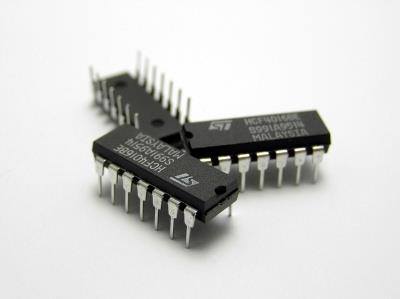
\includegraphics[width=\linewidth]{slike/izvorne/s008_integrisana_kola.jpg}
\end{column}
\begin{column}{.33\textwidth}\centering
\begin{tikzpicture}[font=\fontsize{8}{9.5}\selectfont,x=8mm,y=6mm]
\draw[DEvod] (0,0) rectangle (3,5.4);
\draw[DEvod] (1.15,5.4) arc[start angle=180,end angle=360,x radius=2.8mm,y radius=1.8mm];
\foreach \n/\lab [count=\k] in {1/A_0,2/B_0,3/O_0,4/A_1,5/B_1,6/O_1,7/\mathrm{GND}}{
 \coordinate (p\n) at (0,{5.2-.65*\k});
 \draw[DEvod] (p\n)--++(-.5,0) node[left] {\(\lab\)};
 \node[above,inner sep=1pt] at (-.22,{5.2-.65*\k}) {\n};
}
\foreach \n/\lab [count=\k] in {14/V_{\mathrm{CC}},13/A_2,12/B_2,11/O_2,10/A_3,9/B_3,8/O_3}{
 \coordinate (p\n) at (3,{5.2-.65*\k});
 \draw[DEvod] (p\n)--++(.5,0) node[right] {\(\lab\)};
 \node[above,inner sep=1pt] at (3.22,{5.2-.65*\k}) {\n};
}
\foreach \name/\xx/\yy in {a/1/3.8,b/1/1.7,c/2/3.15,d/2/1.05}{
 \node[and gate US,draw,rotate=-90,logic gate inputs=nn,minimum width=4mm,minimum height=4mm] (\name) at (\xx,\yy) {};
}
\draw[DEvod] (p1)-|(a.input 1) (p2)--++(.4,0)|-(a.input 2) (a.output)|-(p3);
\draw[DEvod] (p4)-|(b.input 1) (p5)--++(.4,0)|-(b.input 2) (b.output)|-(p6);
\draw[DEvod] (p13)-|(c.input 1) (p12)--++(-.4,0)|-(c.input 2) (c.output)|-(p11);
\draw[DEvod] (p10)-|(d.input 1) (p9)--++(-.4,0)|-(d.input 2) (d.output)|-(p8);
\end{tikzpicture}

\end{column}
\begin{column}{.35\textwidth}\centering
\begin{tikzpicture}[font=\fontsize{8}{9.5}\selectfont,x=1.7mm,y=1.25mm]
% Pogled odozgo, 14 izvoda.
\draw[DEvod] (0,15)--(0,18.1) arc[start angle=-90,end angle=90,radius=.45]--(0,22.11)--(19.94,22.11)--(19.94,15)--cycle;
\foreach \i in {0,...,6}{
 \pgfmathsetmacro{\x}{2.0+2.54*\i}
 \draw[DEvod] (\x,15)--++(0,-.5)--++(1.25,0)--++(0,.5);
 \draw[DEvod] (\x,22.11)--++(0,.5)--++(1.25,0)--++(0,-.5);
 \pgfmathtruncatemacro{\n}{\i+1}
 \node[DEcrvena,below,inner sep=1pt] at (\x+.625,14.5) {\n};
 \pgfmathtruncatemacro{\n}{14-\i}
 \node[DEcrvena,above,inner sep=1pt] at (\x+.625,22.61) {\n};
}
\draw[DEzelena] (20.3,15)--(23.5,15) (20.3,22.11)--(23.5,22.11);
\draw[DEzelena,<->] (22.7,15)--(22.7,22.11) node[midway,right,inner sep=1pt] {7.11};
% Bočni pogled i dimenzije iz originala.
\draw[DEvod] (0,4)--(0,8.5)--(19.94,8.5)--(19.94,4);
\draw[DEvod] (0,6.5)--(19.94,6.5);
\foreach \i in {0,...,6}{
 \pgfmathsetmacro{\x}{1.9+2.54*\i}
 \draw[DEvod,fill=white] (\x,4)--(\x,6.2)--++(.4,.3)--++(1.0,0)--++(.35,-.3)--++(0,-2.2)--++(-.4,-.5)--++(0,-2.6)--++(-.95,0)--++(0,2.6)--cycle;
}
\draw[DEzelena] (0,8.8)--(0,11) (19.94,8.8)--(19.94,11);
\draw[DEzelena,<->] (0,10.3)--(19.94,10.3) node[midway,above,inner sep=1pt] {19.94};
\draw[DEzelena] (20.3,8.5)--(24,8.5) (20.3,3.42)--(24,3.42);
\draw[DEzelena,<->] (23,3.42)--(23,8.5) node[midway,right,inner sep=1pt] {5.08};
\draw[DEzelena] (20.3,.88)--(24,.88);
\draw[DEzelena,<->] (21.5,.88)--(21.5,3.42) node[midway,right,inner sep=1pt] {2.54};
\draw[DEzelena] (2.775,.5)--(2.775,-2) (5.315,.5)--(5.315,-2);
\draw[DEzelena,<->] (2.775,-1.5)--(5.315,-1.5);
\node[DEzelena,below,inner sep=1pt] at (5,-1.5) {2.54};
\node[below] at (10,-3.8) {14-Pin DIP};
\end{tikzpicture}
\\
inch=25.4mm\\
mils=inch/1000
\end{column}
\end{columns}
Sa stanovišta minimizacije treba uzeti u obzir ekonomski faktor. U većini slučajeva je ekonomski isplativije kupiti na primer 10000 integrisanih komponenti iste vrste, sa istim sadržajem, nego 5000+5000 komponenti integrisanih komponenti sa različitim sadržajem.
\end{frame}
